\documentclass[12pt,a4paper,twoside]{article}

\setlength{\oddsidemargin}{-0.4mm} % 25 mm left margin - 1 in
\setlength{\evensidemargin}{\oddsidemargin}
\setlength{\topmargin}{-5.4mm} % 20 mm top margin - 1 in
\setlength{\textwidth}{160mm} % 25 mm right margin
\setlength{\textheight}{247mm} % 20 mm bottom margin
\setlength{\headheight}{5mm}
\setlength{\headsep}{5mm}
\setlength{\parindent}{0mm}
\setlength{\parskip}{\medskipamount}
\usepackage{graphicx}
\newcommand{\subsubsubsection}[1]{\vspace{0.01in}\textbf{#1}\vspace{0.01in}\\}
\usepackage{float}
\usepackage{array}
\raggedbottom


\begin{document}

\begin{titlepage}
\begin{center}

\textsc{\LARGE University of Cambridge}\\[3.5cm]

\textsc{\Large Computer Science Tripos \\[2mm] Part 1B Group Project 2013-2014}\\[0.4cm]
\textsc{\Large Team Foxtrot - Money World}\\[2cm]

{\huge \bfseries \vspace{3.5mm} Progress Report}\\[2cm]

\begin{center}
\large
Daniel Low\\
Darren Foong\\
Jovan Powar\\
Samuel Haines\\
\end{center}

\vfill

{\large Last Revised: \today}
\end{center}
\end{titlepage}

\newpage
\thispagestyle{empty}
\cleardoublepage
\newpage

\section{Summary}

Development of the Money World app is going all right except for some minor set backs. 

Firstly, one of our group members has had to leave the group due to personal reasons. As a result, members' tasks had to be reallocated. 

Secondly, The first prototype was delayed because we experienced difficulties setting up the development environment. Some of us were using iPhones and some who were using Android phones were also having issues launching the application on their phones. 

At the time of writing, a prototype has been completed, and will be tested before being demonstrated live at the client meeting on Friday 14 Feb. 
This prototype largely follows the interface described in the specification, with some visualisation models that will be described below.

Subsequent iterations will see more visualisation models, mainly a chart for historical view and a comparison page, and some UI/UX refinements.

Two weeks since the inception of the start of the project, our group has:

\begin{itemize}
	\item Implemented most of the backend for data retrieval.
	\item Implemented a basic user interface to navigate the app.
	\item Developed some visualisation models for use.
\end{itemize}

These will be elaborated in the following sections.

\section{Components}

\subsection{Data retrieval component}
This server-side component has been implemented in Java using the Jersey RESTful Web Services framework with a MySQL database. It is currently running on Google App Engine at \texttt{http://money-world.appspot.com} with a simple API to obtain data in JSON format.

The component executes SQL queries on the MySQL database to obtain Java objects, which are further marshalled into JSON output according to a schema.

The aggregator has not been implemented; currently the database contains only data from the World Bank. Event data for countries will be added to enhance visualisations.

The database schema is as follows:

\begin{itemize}
	\item \textbf{Country} CountryCode, CountryName, Region, IncomeGroup, CountryNotes
	\item \textbf{DataSet} DataSetCode, DataSetName, DataSetNotes, Source
	\item \textbf{DataPoint} DataSetCode, CountryCode, Year, Value,
	\item \textbf{Visualisation} VisualisationID, Type, ExtraData
	\item \textbf{VisualisationCountry} VisualisationID, CountryCode
	\item \textbf{VisualisationDataSet} VisualisationID, DataSetCode
	\item \textbf{Comment} CommentID, CommentBody, CommentUser, VisualisationID, Created, ExtraData
	\item \textbf{CountryCode} CountryCode2, CountryCode3
\end{itemize}

\subsection{Data explanation component}
Not implemented yet (as per project plan).

\subsection{Data visualisation component}
This component's function is to take a set of data and output it in one of the following visualisations.
 
\subsubsection{Map view}
This view will display a world map of the region the country is in (users will have the ability to switch regions if they wish to). For our prototype, the regions are western and southern Africa. Countries in this region will have a colour associated with it which correlates with the economic data currently being visualised.

Navigation around the map is done by panning and using two finger pinching for zooming. This allows the user to select even the smallest country.

The map includes a legends which will appear when a button is pressed, this will give information about what range of values each colour meant.

A population count is displayed at the bottom right. This will display the population of the country when the user hovers (on the computer) or taps (on the phone) on a country. It is represented in a readable form such as "5 million" instead of 5000000.

Maps of different region are separated so that only a particular region is visible on the screen. This is to allow localised comparison. 

A slider is added at the bottom which is used to adjust the year. The map will be redrawn with new data based on the year. 

Testing has been done by visually checking due to the nature of the code produced. Automated unit testing has not been implemented for this as it is small enough to be tested manually.

The following has been visually verified


\begin{itemize}
	\item Values of the indicator corresponds correctly with the colour of the region
	\item Values are updated when the slider change
	\item Legends are updated when there are changes
	\item Population count is transcribed correctly
\end{itemize}


\begin{figure}[H]
\centering
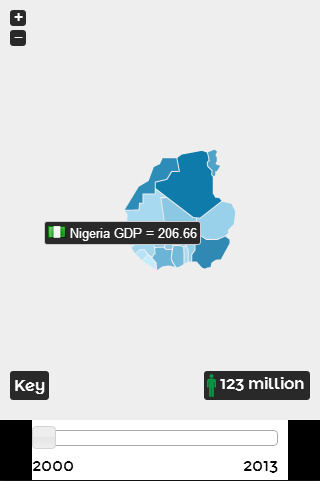
\includegraphics[scale=0.7]{visualisation/map_view.png}
\caption{Map view}
\end{figure}

\subsubsection{Stack View}
This is a view where indicator values are represented by the size of the rectangles. The country with the smallest value will be at the front of the page, and it will be stacked on top of countries with larger values.

The input is a JSON file with a similar format to the one used by the map view. 

The output is automatically generated rectangles identifiable by country flags.


\begin{figure}[H]
\centering
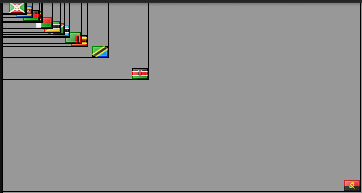
\includegraphics[scale=1]{visualisation/stack_view.png}
\caption{Stack view}
\end{figure}


\subsubsection{Grid view}
After further consideration, this view may not be used at all because it isn't entirely intuitive how the economic data are visualised other than being outputted as text.

This is a view where country's economic data is represented in some manner within individual cells that are automatically generated based on the input given. 

The input is a JSON file with a similar format to the one used by the map view. 

\subsubsection{Bubble chart view}
This view's development is delayed.

\subsubsection{Line chart view}
This view's development is delayed.

\subsection{Comment display and input component}
This component is dropped because we have decided it was unnecessary during the first client meeting. This is combined with the sharing component.

\subsection{Comment storage component}
This component is dropped because we have decided it was unnecessary during the first client meeting. This is combined with the sharing component.

\subsection{Sharing component}
Not implemented yet (as per project plan).

\subsection{UI and UX component}
The frontend runs on the Sencha Touch framework and Cordova to run on Android phones. A basic user interface has been implemented that can easily incorporate visualisations. Basic user details can be stored and retrieved for the application's purposes (country, region).

Further improvements required are styling and theming of the interface, with extra graphics and icons to enhance the apperance.

The frontend is build according to the Model-View-Controller (MVC framework). As of writing, the components are:

\begin{itemize}
	\item \textbf{Models} Setting, Country
	\item \textbf{Views} Init, Main, Settings, Overview, DetailedView, ComparisonView, MainTileView, MapView
	\item \textbf{Controllers} Init, Main, Settings, Overview, MainTileView, MapView
	\item \textbf{Stores} Settings, Countries
\end{itemize}

\end{document}
